\subsection{Verkenning van afdekking en onzekere handpunten}\label{app:gh-occlusion}
\paragraph{Twee verschillende benaderingen.}
Een skeletrotatie houdt alle 21 punten intact. Om afdekking te benaderen, bouwen we rond de bestaande punten een grof volumemodel: een ellipsoïde voor de palm en taps toelopende buisjes met ronde uiteinden voor de vingers. Een dieptebuffer bepaalt welk handdeel vooraan ligt. Vingerbreedte, palmdikte, kleur, licht en achtergrond zijn vaste aannames; er is geen anatomische passing of nieuwe foto. De geometrie gebruikt geen letterlabel. De aanname dat de bron de palmzijde toont, is evenmin voor alle bronnen gecontroleerd.

Op 64 vooraf geselecteerde bronnen (32 G, 32 H) accepteert MediaPipe alle oorspronkelijke foto's. Zowel zonder als met halve draai wordt geen van de 64 renders als hand geaccepteerd: nul van 128 synthetische beelden. Detectie- en aanwezigheidsdrempel staan beide op 0,5. Deze renderroute levert dus geen nieuwe detectorlandmarks voor training op. We vervangen mislukte detecties niet door de bekende bronpunten.

\paragraph{Afzonderlijke robuustheidsproef.}
We bewerken daarnaast de landmarks rechtstreeks. Van alle 4.801 G/H-bronnen draaien we de beeld- en wereldpunten om de pols. Bij PIP-, DIP-, IP- en duimpunten die volgens de dieptebuffer achter een \emph{ander} handdeel liggen, voegen we normaalverdeelde verstoring toe. De standaardafwijking per coördinaat is vooraf vastgezet op 2\% of 5\% van de pols--middelvingerknokkelafstand. Hetzelfde gelote patroon wordt op beide coördinatenbronnen toegepast, met hun eigen schaal. Niet geselecteerde punten, pols en vingerknokkels blijven exact op hun gedraaide plaats. Dit benadert onzekere puntposities; het is geen gemeten model van fouten die MediaPipe bij afdekking maakt. Ook zelfafdekking binnen één vinger wordt niet gemodelleerd.

Per bron gebruiken beide sterktes hetzelfde reproduceerbare ruispatroon. Alle 835 features worden herberekend; de nulverstoring reproduceert voor alle 4.801 bronnen de bestaande rotatie binnen $10^{-5}$. De oorspronkelijke G/H-rij en één bewerkte kopie wegen elk 0,5. Dezelfde vijf bronblokken, oorspronkelijke preprocessing, numerieke SVM-gamma en klassegewichten blijven behouden. Alleen trainingsbronnen leveren trainingskopieën; er worden geen webcamopnamen gebruikt.

\begin{table}[h]\centering\small
\caption{Regressiecontrole op 60.251 oorspronkelijke, geaccepteerde toetsbeelden. P is macro-precisie (\%). Herstel/verlies is gepaard tegenover de oorspronkelijke training. Dit is geen handrugtoets.}
\begin{tabular}{lrrrr}\toprule
Training & P (\%) & Macro-F1 & Correct & Herstel/verlies\\\midrule
\tableinput occlusion_results_nl.tex
\bottomrule\end{tabular}
\end{table}

The 2\% arm exactly matches pure-rotation predictions on originals; the 5\% arm loses one additional correct prediction. Neither adds an original-view gain. This does not validate the noisy points as realistic hand-back observations.


\paragraph{Aanvullende kunstmatige toets.}
In een afzonderlijke controle draaien we \emph{uitsluitend de G/H-toetslandmarks} van dezelfde bronblokken; de andere 24 letters blijven oorspronkelijk. De modellen worden niet opnieuw getraind. Deze toets maakt zichtbaar of de toegevoegde geometrie geleerd wordt, maar maakt van geschatte punten geen echte handrugdetectie.

\begin{table}[h]\centering\small
\caption{Kunstmatige toets: G/H-landmarks gedraaid, overige letters ongewijzigd. Dezelfde 60.251 bronnen; geen nieuwe RGB-detecties.}
\begin{tabular}{lrrr}\toprule
Training & P (\%) & Macro-F1 & Correct\\\midrule
Oorspronkelijk & 85.0689 & 0.869284 & 54.151 \\
Alleen rotatie & 97.5861 & 0.975715 & 58.924 \\
Rotatie + 2\% puntverstoring & 97.5830 & 0.975683 & 58.922 \\
Rotatie + 5\% puntverstoring & 97.5802 & 0.975653 & 58.920 \\
\bottomrule\end{tabular}\end{table}
Met alleen rotatie worden netto 4.773 extra letters goed herkend ten opzichte van de oorspronkelijke training. De recall op de gedraaide G/H-punten stijgt van 0\% / 0,04\% naar 99,47\% / 99,45\%. De puntverstoring geeft ook in deze controle geen extra winst. De rotatie leert dus de aangeboden geometrie, terwijl de vrijwel gelijke oorspronkelijke score alleen behoud op het oude aanzicht beschrijft.


\clearpage
\subsection{Geschatte afdekking in beeld}
De onderstaande beelden maken de geometrische aannames zichtbaar. De bronfoto's zijn dezelfde twee voorbeelden als in figuur~\ref{fig:gh-training-rotation}; de volumes zijn uit hun opgeslagen handpunten opgebouwd. Een rode cirkel geeft een positie achter een ander volumedeel aan. De plaats van zo'n punt blijft bekend uit de bron; een echte detector zou die plaats opnieuw moeten schatten.

\begin{figure}[h]\centering
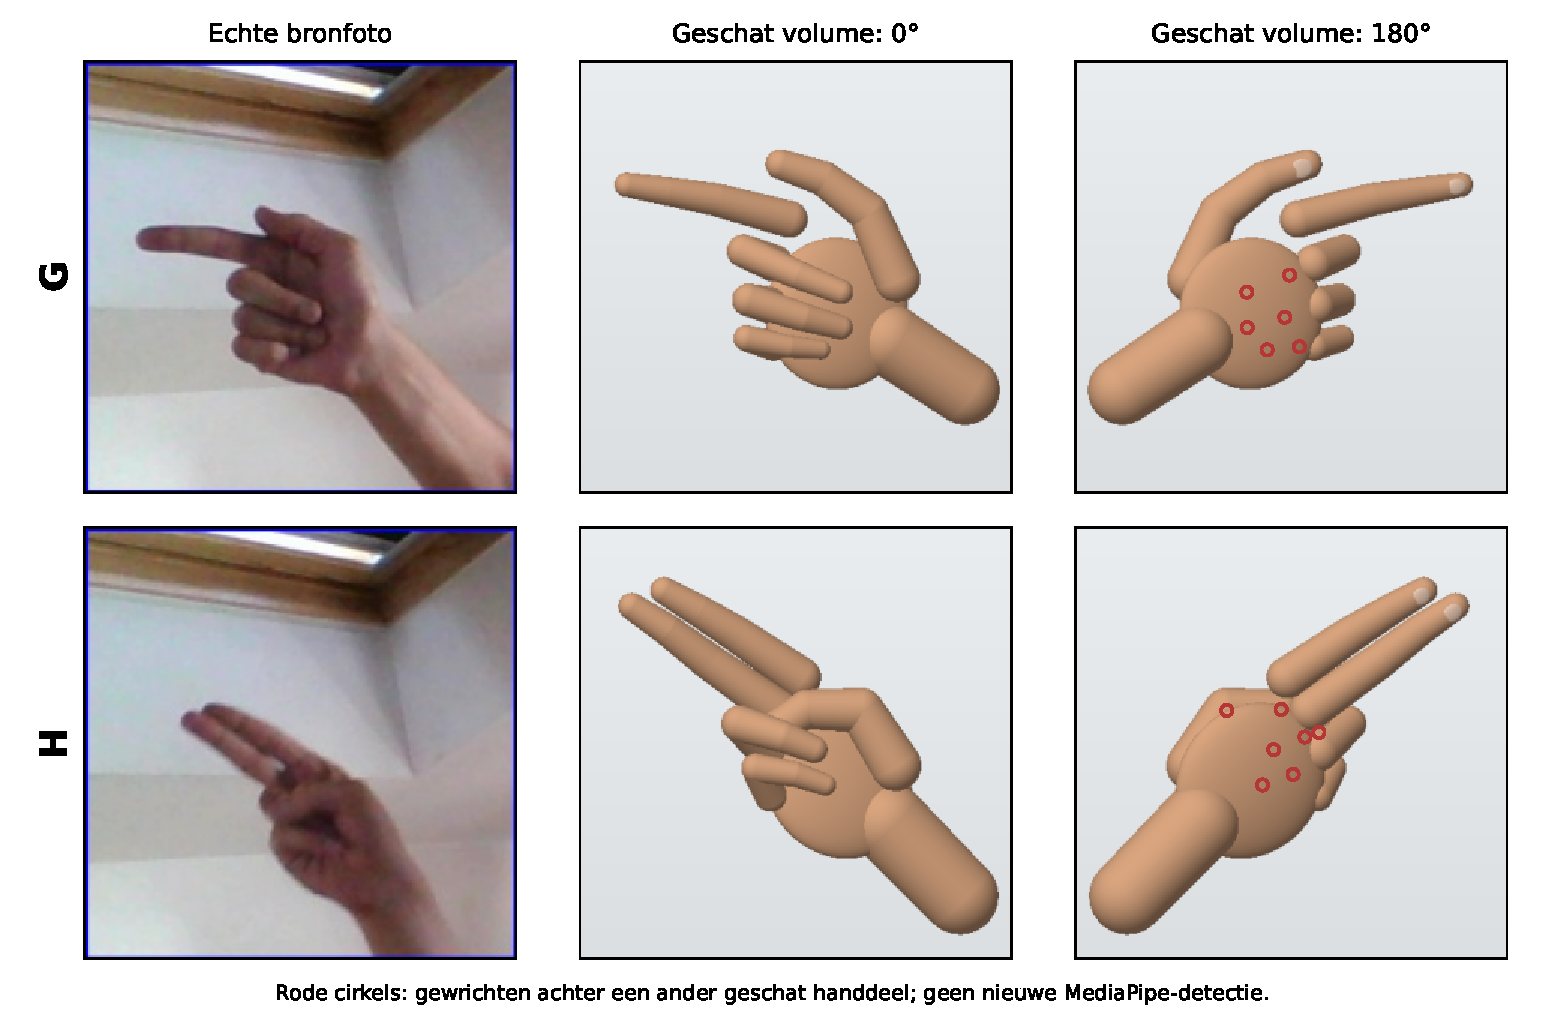
\includegraphics[width=.77\linewidth]{figures/gh_occlusion_proxy.pdf}
\caption{Twee vaste trainingsvoorbeelden en hun geschatte volumes. Rode cirkels markeren punten achter een ander volumedeel. Het zijn illustraties van de aannames; de gerenderde hand is geen nieuwe waarneming. MediaPipe vindt in deze renders geen hand.}
\label{fig:gh-occlusion-proxy}
\end{figure}

De protocollen, bronselectie, vijf folds, per-letterresultaten en voorspellingen staan met hashes in \path{results/gh_occlusion_01/}. De bestaande dataset is eerder tijdens ontwikkeling bekeken. Beide ruissterktes zijn verkennend; er wordt geen winnaar als nieuwe live-standaard gekozen. Voor de gewenste ASL-uitvoering blijft een onafhankelijk gecontroleerde handrugtoets nodig, waarbij detectiemislukkingen ook meetellen.
